% !TeX TXS-program:compile = txs:///pdflatex/[--shell-escape]
\documentclass[]{article}
\usepackage{polski}
\usepackage[utf8]{inputenc}
\usepackage{graphicx}
\usepackage{wrapfig}
\usepackage{float}
\graphicspath{{./zdjecia/}}


% Title Page
\title{Sprawozdanie Lab 3}
\author{Wojciech Kosierkiewicz 272926}
%python config
% !TeX TXS-program:compile = txs:///pdflatex/[--shell-escape]
\usepackage{tcolorbox}
\tcbuselibrary{minted,breakable,xparse,skins}

\definecolor{bg}{gray}{0.95}
\DeclareTCBListing{mintedbox}{O{}m!O{}}{%
  breakable=true,
  listing engine=minted,
  listing only,
  minted language=#2,
  minted style=default,
  minted options={%
    linenos,
    gobble=0,
    breaklines=true,
    breakafter=,,
    fontsize=\small,
    numbersep=8pt,
    #1},
  boxsep=0pt,
  left skip=0pt,
  right skip=0pt,
  left=25pt,
  right=0pt,
  top=3pt,
  bottom=3pt,
  arc=5pt,
  leftrule=0pt,
  rightrule=0pt,
  bottomrule=2pt,
  toprule=2pt,
  colback=bg,
  colframe=orange!70,
  enhanced,
  overlay={%
    \begin{tcbclipinterior}
    \fill[orange!20!white] (frame.south west) rectangle ([xshift=20pt]frame.north west);
    \end{tcbclipinterior}},
  #3}

% !TeX TXS-program:compile = txs:///pdflatex/[--shell-escape]


\begin{document}
	\maketitle
	\newpage
	
\section{Wstęp}
Podczas tych laboratoriów uczyłem się operowania wirtualną kamerą w środowisku 3D. W zadaniach musiałem ustawiać kamerę w różnych miejsca i pod różnymi kątami. Do sterowania jej używałem danych z ruchu myszką i sygnałów klawiatury.
\section{Zadania}
\subsection{zadanie 1}
W miałem przestudiować obrót kamerą w poziomie i dodać możliwość obrotu w pionie
\begin{figure}[H]
	\begin{minted}{python}
def render(time):
    global theta
    global phi

    glClear(GL_COLOR_BUFFER_BIT | GL_DEPTH_BUFFER_BIT)
    glLoadIdentity()

    gluLookAt(viewer[0], viewer[1], viewer[2],
              0.0, 0.0, 0.0, 0.0, 1.0, 0.0)

    if left_mouse_button_pressed:
        theta += delta_x * pix2angle
        phi += delta_y * pix2angle

    glRotatef(theta, 0.0, 1.0, 0.0)
    glRotatef(phi, 1.0, 0.0, 0.0)

    axes()
    example_object()

    glFlush()
\end{minted}
\caption{Kod obsługujący kamery wokół obiektu obiektu}
\end{figure}
\begin{figure}[H]

	\centering
	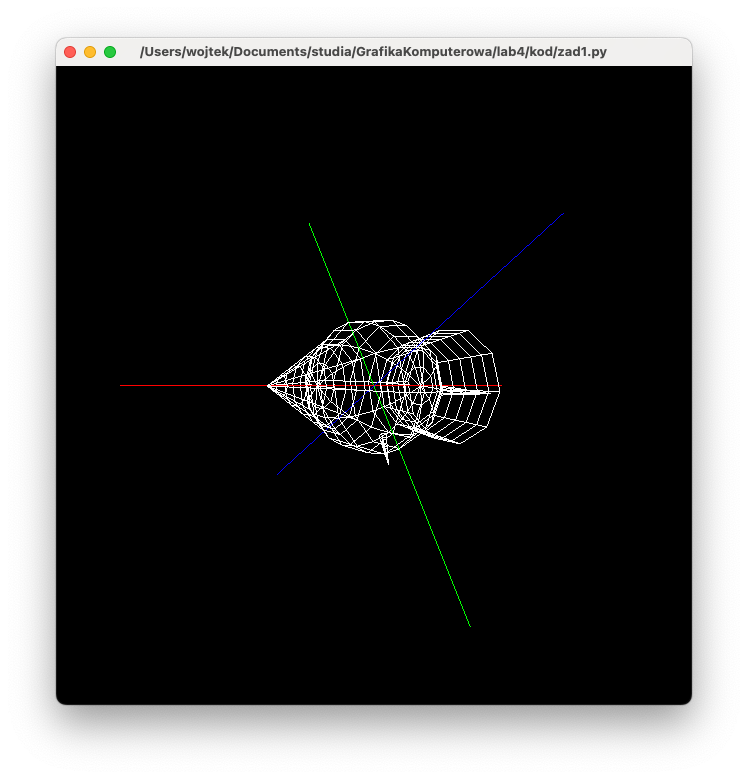
\includegraphics[width=\textwidth]{zad1.png}
	\caption{Wynik zadania 1}
\end{figure}
\subsection{zad2}
W następnym zadaniu miałem jeszcze dodać opcje skalowania skalowania naszego obiektu po przyciśnięciu guzika myszy. Do wykonania tego zmieniałem albo thete i phi na podstawie myszki lub scale zależnie od nacisniętego guzika. Dodałem także wywołanie glScalef które było odpowiedzialne za odpowiednie przeskalowanie.
\begin{figure}[H]
	\begin{minted}{python}
def render(time):
    global theta
    global phi
    global scale
    global scale

    glClear(GL_COLOR_BUFFER_BIT | GL_DEPTH_BUFFER_BIT)
    glLoadIdentity()

    gluLookAt(viewer[0], viewer[1], viewer[2],
              0.0, 0.0, 0.0, 0.0, 1.0, 0.0)

    if left_mouse_button_pressed:
        theta += delta_x * pix2angle
        phi += delta_y * pix2angle

    if right_mouse_button_pressed:
        scale += delta_y * 0.01
        scale += delta_x * 0.01

    glRotatef(theta, 0.0, 1.0, 0.0)
    glRotatef(phi, 1.0, 0.0, 0.0)
    glScalef(scale,scale,scale)

    axes()
    example_object()

    glFlush()
	\end{minted}
\end{figure}
\begin{figure}[H]

	\centering
	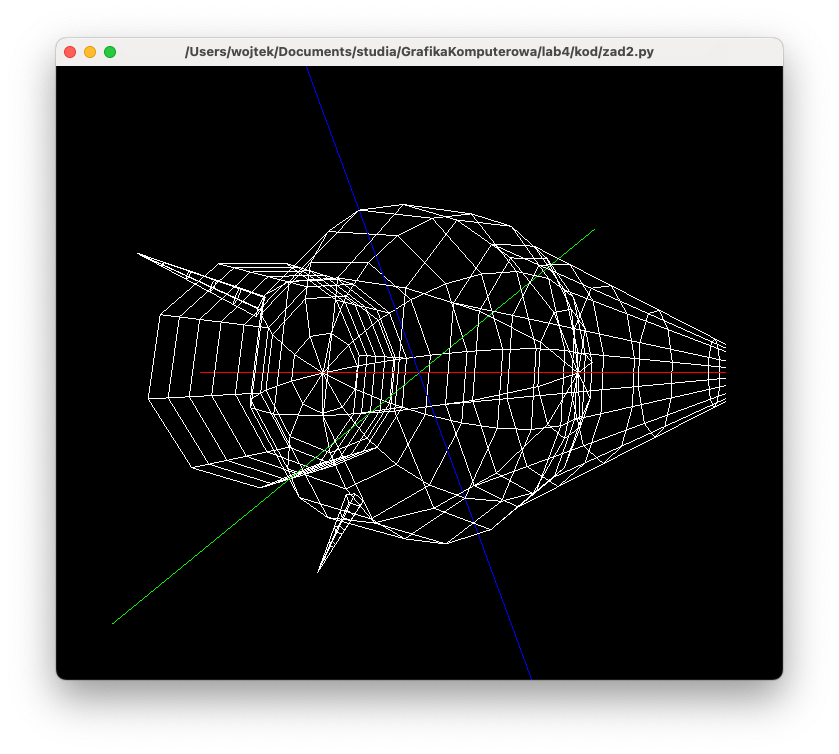
\includegraphics[width=\textwidth]{zad2.png}
	\caption{Wynik zadania 2}
\end{figure}

\subsection{zad3}
W zadaniu 3 musiałem wykonać pełny obrót kamery wokół obiektu przy obliczaniu $x_{eye}$ $y_{eye}$ i  $z_{eye}$

\begin{figure}[H]
	\begin{minted}{python}
def render(time):
    global theta
    global phi
    global scale
    global r

    glClear(GL_COLOR_BUFFER_BIT | GL_DEPTH_BUFFER_BIT)
    glLoadIdentity()
    
    if left_mouse_button_pressed:
        theta += delta_x * pix2angle
        phi += delta_y * pix2angle


    if right_mouse_button_pressed:
        r += delta_y * pix2angle
        r += delta_x * pix2angle

    xeye=r*sin(theta*pi/180)*cos(phi*pi/180)
    yeye=r*sin(phi*pi/180)
    zeye=r*cos(theta*pi/180)*cos(phi*pi/180)

    gluLookAt(xeye, yeye, zeye, 0.0, 0.0, 0.0, 0.0, 1.0, 0.0)


    axes()
    example_object()

    glFlush()
	\end{minted}
\end{figure}
\begin{figure}[H]

	\centering
	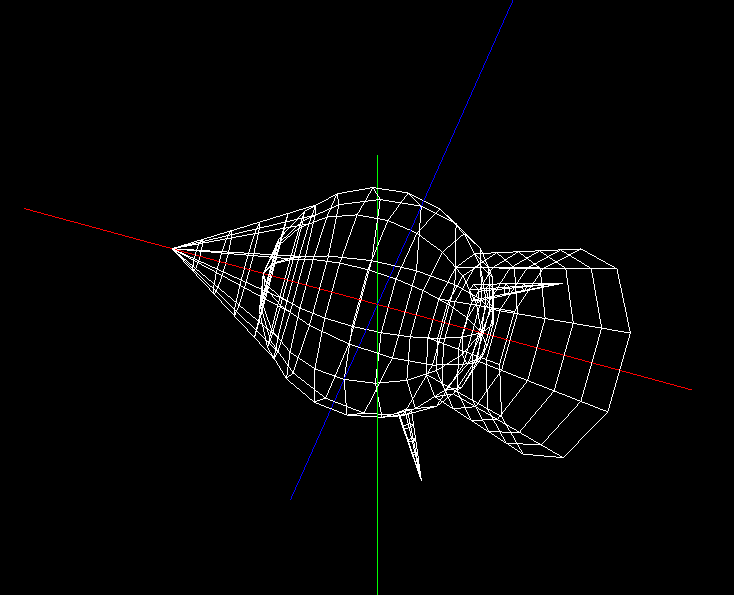
\includegraphics[width=\textwidth]{zad3.png}
	\caption{Wynik zadania 3}
\end{figure}

\subsection{zad4}
W zadaniu 4 musiałem dodać limity obrotu dzięki którym nie możliwe było obrócenie przedmiotu ponad zakres logiczny. dlatego dla osi poziomej ustawiłem maksymalny kąt 360 stopni a dla osi pionowej obrót o $-90^o$ i $90^o$.
\begin{figure}[H]
	\begin{minted}{python}
def render(time):
    global theta
    global phi
    global thetas
    global phis
    global scale
    global r
    global xeye, yeye, zeye
    global objclrx, objclry, objclrz

    glClear(GL_COLOR_BUFFER_BIT | GL_DEPTH_BUFFER_BIT)
    if (moving == "camera"):
        objclrx = 1.0
        objclry = 1.0
        objclrz = 1.0
    else:
        objclrx =0.0
        objclry = 1.0
        objclrz = 1.0
    glLoadIdentity()
    
    if (moving == "camera"):
        xeye=r*sin(theta*pi/180)*cos(phi*pi/180)
        yeye=r*sin(phi*pi/180)
        zeye=r*cos(theta*pi/180)*cos(phi*pi/180)
        if left_mouse_button_pressed:
            theta += delta_x * pix2angle
            phi += delta_y * pix2angle
            phi = max(-90.0, min(90.0, phi))
            theta = fmod(theta, 360.0)
        if right_mouse_button_pressed:
            r += delta_y * pix2angle
            r += delta_x * pix2angle
            r = max(1.0, abs(r))
            r = min(10.0, abs(r))
    else:
        if left_mouse_button_pressed:
            thetas += delta_xs * pix2angle
            phis += delta_ys * pix2angle

        if right_mouse_button_pressed:
            scale += delta_ys * pix2angle/100
            scale += delta_xs * pix2angle/100

    gluLookAt(xeye, yeye, zeye, 0.0, 0.0, 0.0, 0.0, 1.0, 0.0)
    glRotatef(thetas, 0.0, 1.0, 0.0)
    glRotatef(phis, 1.0, 0.0, 0.0)
    glScalef(scale,scale,scale)

    axes()
    example_object()

    glFlush()
	\end{minted}
\end{figure}
\end{document}          
